\documentclass[a4paper, 12pt]{article}

\usepackage[italian]{babel}
\usepackage[utf8]{inputenc}
\usepackage[T1]{fontenc}
\usepackage{graphicx}
\usepackage{geometry}
\usepackage{float}
\usepackage{tabularx}
\usepackage{listings}
\usepackage{xcolor}

% Colori coerenti con l'immagine
\definecolor{sqlgreen}{rgb}{0,0.5,0}
\definecolor{sqlblack}{rgb}{0,0,0}
\definecolor{sqlblue}{rgb}{0,0,0.7}
\definecolor{sqlpurple}{rgb}{0.58,0,0.82}
\definecolor{sqlgray}{rgb}{0.5,0.5,0.5}
\definecolor{sqlbg}{rgb}{0.98,0.98,0.98}

\lstdefinestyle{sqlstyle}{
	language=SQL,
	backgroundcolor=\color{sqlbg},
	basicstyle=\footnotesize\ttfamily,
	commentstyle=\color{sqlgreen}\itshape,
	keywordstyle=\color{sqlblue}\bfseries,
	stringstyle=\color{sqlpurple},
	showstringspaces=false,
	numbers=left,
	numberstyle=\tiny\color{sqlblack},
	numbersep=2pt,
	breaklines=true,
	tabsize=2,
	frame=single,
	rulecolor=\color{black},
	framerule=0.5pt,
	xleftmargin=15pt,
	framexleftmargin=10pt,
	aboveskip=10pt,
	belowskip=10pt,
	morekeywords={
		CREATE, TABLE, PRIMARY, KEY, FOREIGN, REFERENCES,
		CONSTRAINT, CHECK, VARCHAR, INTEGER, DATE, NOT, NULL,
		AND, OR, BEGIN, END, IF, THEN, ELSE, RETURN, DEFAULT
	}
}



\geometry{a4paper, top=2.5cm, bottom=2.5cm, left=3cm, right=3cm}

\begin{document}

\begin{titlepage}
    {
        \centering      % Assicura la centratura
        \scshape        % Applica lo stile Maiuscoletto (Small Caps) a tutto il blocco
        
        {\large {\LARGE U}NIVERSITÀ DEGLI STUDI DI {\LARGE N}APOLI {\LARGE F}EDERICO II\par}
        \vspace{0.25cm}
    
        {\small DIPARTIMENTO DI INGEGNERIA ELETTRICA E TECNOLOGIE DELL'INFORMAZIONE\par}
    }

    \vspace{1cm} 

    \centering
    {
    
\includegraphics[width=4cm]{pics/coverlogo.png}
    }

    \vspace{1cm}

    {
        \scshape
        CORSO DI LAUREA IN INFORMATICA \\[0.5cm]
        INSEGNAMENTO DI BASI DI DATI I \\[0.5cm]
        ANNO ACCADEMICO 2024/2025 \\
    }

    \vfill

    % --- TITOLO PRINCIPALE ---
    {
        \centering 
        \Large\bfseries
        
        Documentazione per \\[1cm]
        Progettazione Schema della Base di Dati \\[0.5cm]
        Ristrutturazione dello Schema secondo il modello relazionale \\[0.5cm]
        Schema Fisico
    }

    \vfill 

    \begin{minipage}[t]{0.4\textwidth}
        \flushleft 
        \underline{Autore:}\\[0.3cm]
        Salvatore DE PASQUALE \\
        MATRICOLA N86005746 \\
        \texttt{salvat.depasquale@studenti.unina.it} \\[0.5cm]
    \end{minipage}
    \hfill 
    \begin{minipage}[t]{0.4\textwidth}
        \flushleft 
        \underline{Docente:}\\[0.3cm]
        Prof.ssa Mara SANGIOVANNI
    \end{minipage}

\end{titlepage}

\newpage

\tableofcontents

\newpage

\section{Introduzione}
    Questo documento descrive le fasi di progettazione della base di dati a supporto del sistema UninaFoodLab, una piattaforma per la gestione di corsi di cucina tematici. Vengono presentati lo Schema della Base di Dati, la ristrutturazione secondo il modello relazionale e lo Schema fisico. Questo documento fa parte del progetto BDD+OOP, riguardante i corsi di Basi Di Dati I e Programmazione Object-Oriented, a cura di Salvatore De Pasquale, studente del CdL in Informatica presso l'Università degli Studi di Napoli Federico II (gruppo OOBD84).

    \subsection{Traccia del Progetto}
    UninaFoodLab è un sistema per la gestione di corsi di cucina tematici. Gli chef possono registrare corsi su specifici argomenti (es. cucina asiatica, pasticceria, panificazione), specificando una data di inizio e una frequenza delle sessioni (es. settimanale, ogni due giorni). Ogni corso è articolato in più sessioni, che possono essere di due tipi: online, oppure in presenza, in cui gli utenti svolgono attività pratiche. Gli utenti possono iscriversi a più corsi e, nel caso delle sessioni pratiche, devono fornire una adesione esplicita per confermare la loro partecipazione. Ogni sessione pratica prevede la preparazione di una o più ricette, ciascuna delle quali richiede una specifica lista di ingredienti. Le adesioni vengono utilizzate per pianificare correttamente la quantità di ingredienti necessari, evitando cosi sprechi alimentari. Si utilizzino le proprie conoscenze del dominio per definire eventuali dettagli non specificati nella traccia.

    \subsection{Obiettivi}
    Gli obiettivi principali della base di dati sono:
    \begin{itemize}
        \item \textbf{Memorizzare} in modo strutturato tutte le informazioni relative a chef, utenti, corsi, sessioni, e ricette.
        \item \textbf{Definire} le relazioni tra le entità.
        \item \textbf{Garantire} integrità dei dati, attraverso l'uso di vincoli.
        \item \textbf{Supportare} le query necessarie al calcolo esatto delle quantità di ingredienti in merito al numero di partecipanti che confermano la presenza per ogni sessione pratica.
    \end{itemize}
  
\newpage

\section{Progettazione schema della base di dati}
    Basandoci sulla traccia assegnata, definiamo le entità e le relazioni che le collegano. Questo ci porterà a definire lo schema del nostro database.

    \subsection{Entità Principali}
    \begin{itemize}
        \item \textbf{Chef}: Chi tiene i corsi.
        \item \textbf{Utente}: Chi si iscrive ai corsi.
        \item \textbf{Corso}: L'argomento generale di studio (es. Pasticceria).
        \item \textbf{Sessione}: Una singola lezione di un corso.
        \item \textbf{Ricetta}: Una preparazione specifica insegnata in una sessione.
        \item \textbf{Ingrediente}: Un componente di una ricetta.
    \end{itemize}

    \subsection{Relazioni e Cardinalità}
    \begin{itemize}
        \item Uno Chef può creare molti Corsi. Un Corso è tenuto da un solo Chef (Relazione 1 a N).
        \item Un Utente può iscriversi a diversi Corsi, e un Corso può avere molti Utenti (Relazione N a N e conseguente entità derivata "Iscrizione").
        \item Un Corso si articola in più Sessioni. Ogni Sessione appartiene ad un solo Corso (Relazione 1 a N).
        \item Una Sessione è esattamente di un tipo: online o in presenza (Deduciamo che avrà una relazione 1 a 1 con una delle sotto-entità "SessioneOnline" e "SessioneInPresenza". Questa, ovviamente, risulta essere una \textit{generalizzazione}, esclusiva e totale).
        \item Un Utente da l'adesione a più Sessioni in presenza, mentre una Sessione in presenza riceve l'adesione da più Utenti (Relazione N a N, deduciamo che abbiamo quindi l'entità derivata "Adesione").
        \item Una Sessione in presenza include la preparazione di molte Ricette, una Ricetta può far parte di più Sessioni (Relazione N a N, ne consegue quindi "ProgrammaSessione").
        \item Una Ricetta è composta da molti Ingredienti, un Ingrediente può essere usato in più Ricette (Relazione N a N, abbiamo quindi "ComposizioneRicetta" derivata).
    \end{itemize}

    \newpage
    \subsection{Diagramma ER (Entità Relazione)}
    \begin{figure}[H]
        \centering
        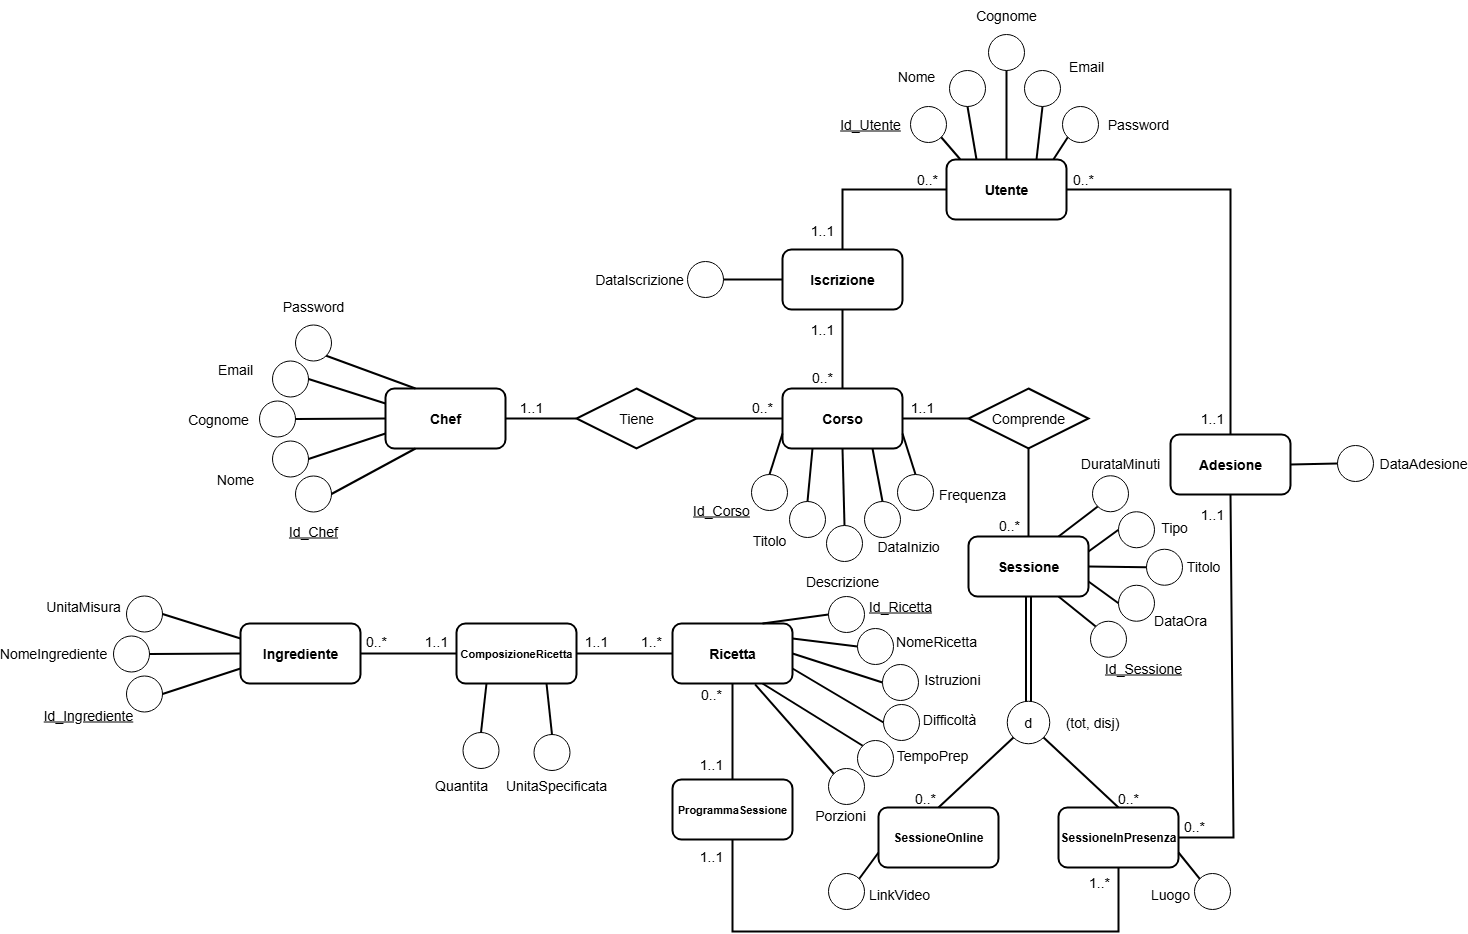
\includegraphics[width=1\linewidth]{pics/DiagrammaEERProgetto.png}
        \caption{\label{fig:DiagrammaEERProgetto}Diagramma Entità Relazione Esteso}
    \end{figure}

    Il diagramma mostrato in figura fornisce una visione astratta e formale delle informazioni, gestite dalle loro entità e relazioni che pongono le basi per la successiva progettazione logica e fisica della base di dati.\\[0.3cm]
    La modellazione ha permesso di identificare le seguenti entità principali:
    \begin{itemize}
        \item Entità anagrafiche, come Chef e Utente, che sono gli attori del sistema.
        \item Entità centrali, come Corso, Sessione, Ricetta, e Ingrediente.
    \end{itemize}
    Per descrivere in modo completo il dominio, sono state implementate le seguenti relazioni e gestioni di queste ultime:
    \begin{itemize}
        \item Relazioni Uno-a-Molti (1..N): Legami più diretti, come quelli, ad esempio, tra Chef e Corso, sono stati modellati specificando le relative cardinalità, secondo le regole comuni dei modelli ER.
        \item Relazioni Molti-a-Molti (N..M): Per gestire queste complesse relazioni sono state implementate le entità associative, come:
            \begin{itemize}
                \item Iscrizione
                \item ComposizioneRicetta
                \item Adesione
                \item ProgrammaSessione
            \end{itemize}
        Ognuna con i propri eventuali attributi. Necessarie ai fini del corretto funzionamento logico del sistema.
        \item Generalizzazione/Specializzazione: L'entità Sessione è stata generalizzata, producendo due entità più specifiche: SessioneOnline e SessioneInPresenza. Questa scelta è dovuta, ovviamente, al fatto che una Sessione di un Corso può essere unicamente una delle due opzioni. La relazione è totale e disgiunta, significando che deve obbligatoriamente essere di uno e un solo tipo.
    \end{itemize}

    \subsection{Diagramma Delle Classi UML}
    \begin{figure}[H]
        \centering
        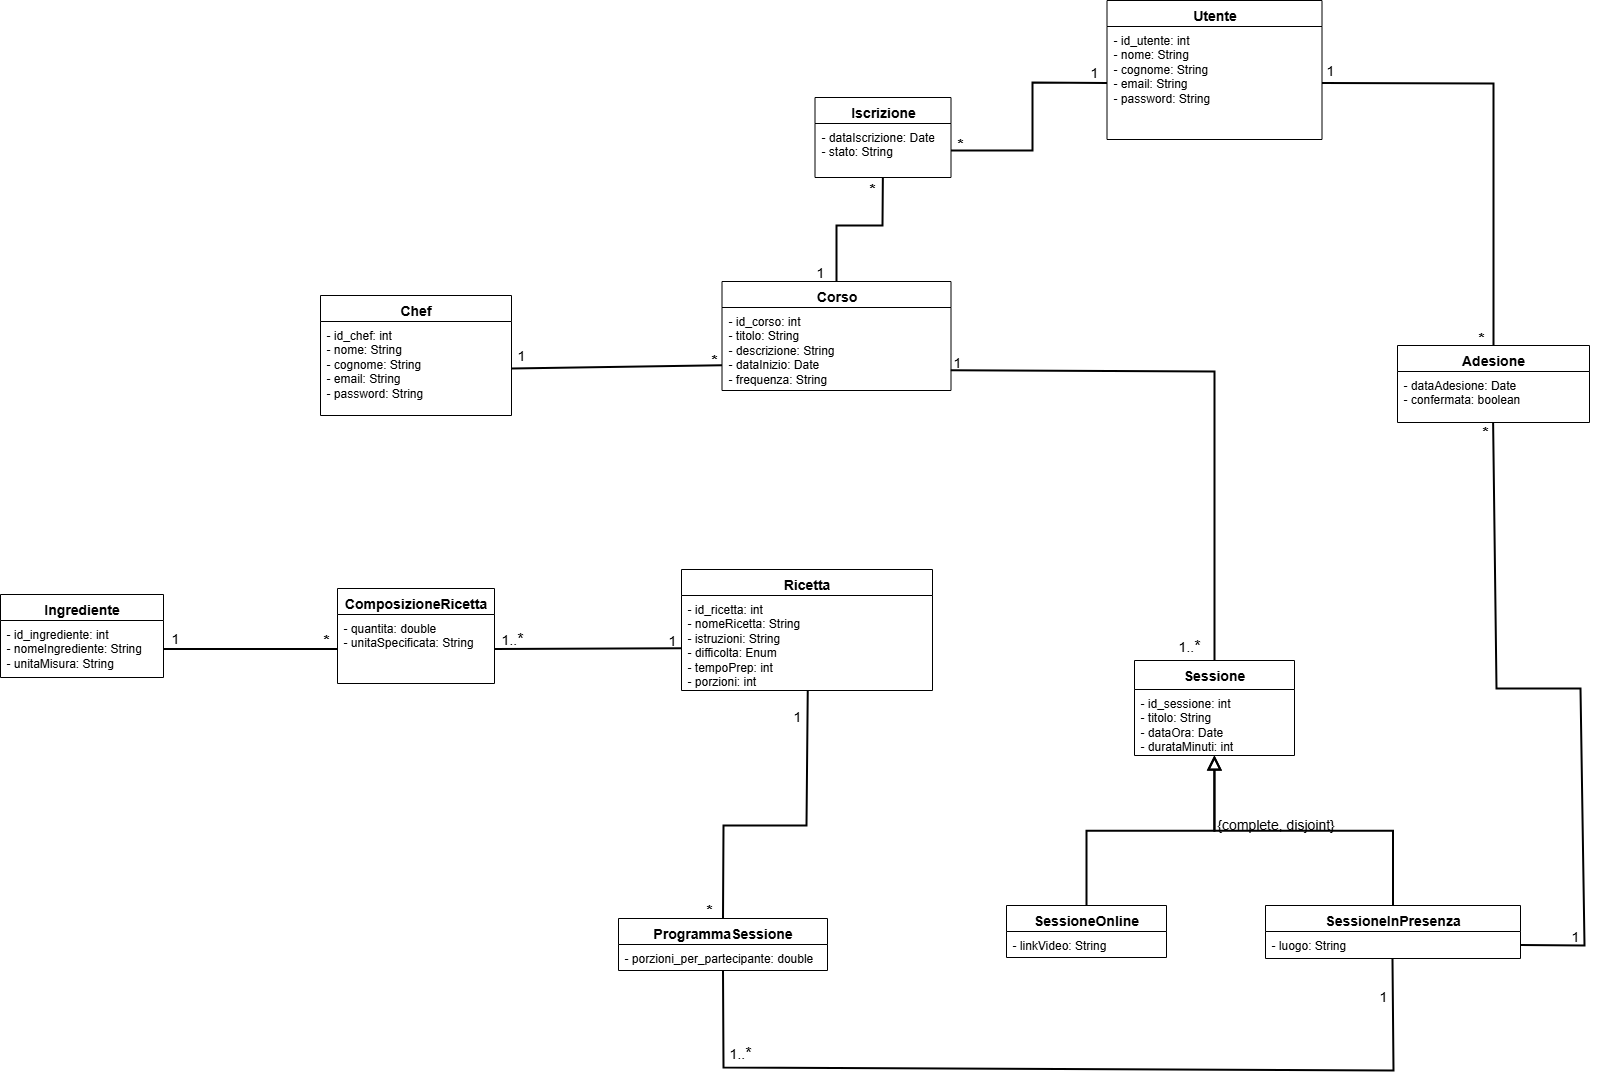
\includegraphics[width=1\linewidth]{pics/DiagrammaClassiUML.png}
        \caption{\label{fig:DiagrammaClassiUML}Diagramma delle Classi UML}
    \end{figure}
    Procediamo quindi adesso con la conversione del diagramma EER nel diagramma UML, una versione quindi meno vaga e più organizzata, che, una volta ristrutturato, sarà un ottimo blueprint per la progettazione vera e propria della base di dati.\\[0.3cm]
    Il modello EER è stato tradotto seguendo criteri specifici, privilegiando l'incapsulamento, l'ereditarietà, e una corretta rappresentazione delle associazioni tra gli oggetti.\\[0.3cm]
    Analizziamo quali regole e criteri sono stati seguiti per la corretta conversione:
    \begin{itemize}
        \item Entità e Classi: Anzitutto, ogni entità del modello è stata tradotta in classe. Le entità associative, inoltre, vengono rappresentate come classi vere e proprie, in quanto rappresentano concetti con propri attributi e comportamenti.
        \item Attributi e Incapsulamento: Gli attributi di ogni entità sono stati trasformati in attributi privati, con un tipo di dato specifico (es. String, int, Date). Questa scelta implementa il principio di incapsulamento, proteggendo i dati.
        \item Specializzazione e Ereditarietà: La generalizzazione dell'entità Sessione è stata tradotta correttamente utilizzando l'ereditarietà. La Classe "padre" Sessione nel dominio non esiste, una "sessione generica" non è una scelta possibile, ma deve piuttosto essere sempre online o in presenza.
            \begin{itemize}
                \item Polimorfismo: Questo approccio ci consente di gestire le sessioni in maniera polimorfica. Ad esempio, la classe Corso potrebbe contenere una lista di sessioni e gestire gli oggetti al suo interno senza conoscere il loro tipo specifico, delegando la cosa alle sottoclassi.
                \item Vincolo: il vincolo di generalizzazione scelto è "{complete, disjoint}", sempre per i motivi elencati sopra.
            \end{itemize}
    \end{itemize}

\section{Ristrutturazione secondo il modello relazionale}
    Dopo aver definito il modello tramite il diagramma delle classi UML (versione concettuale), in questo capitolo si illustra il processo di ristrutturazione che porta alla versione UML ristrutturata, pronta per la traduzione nello schema logico relazionale.\\[0.2cm]
    L'obiettivo è di ridefinire il modello, perfezionandolo in fatto di compatibilità con il linguaggio SQL in modo tale da permetterci una conversione più semplice, veloce, e coerente.

    \begin{figure}[H]
        \centering
        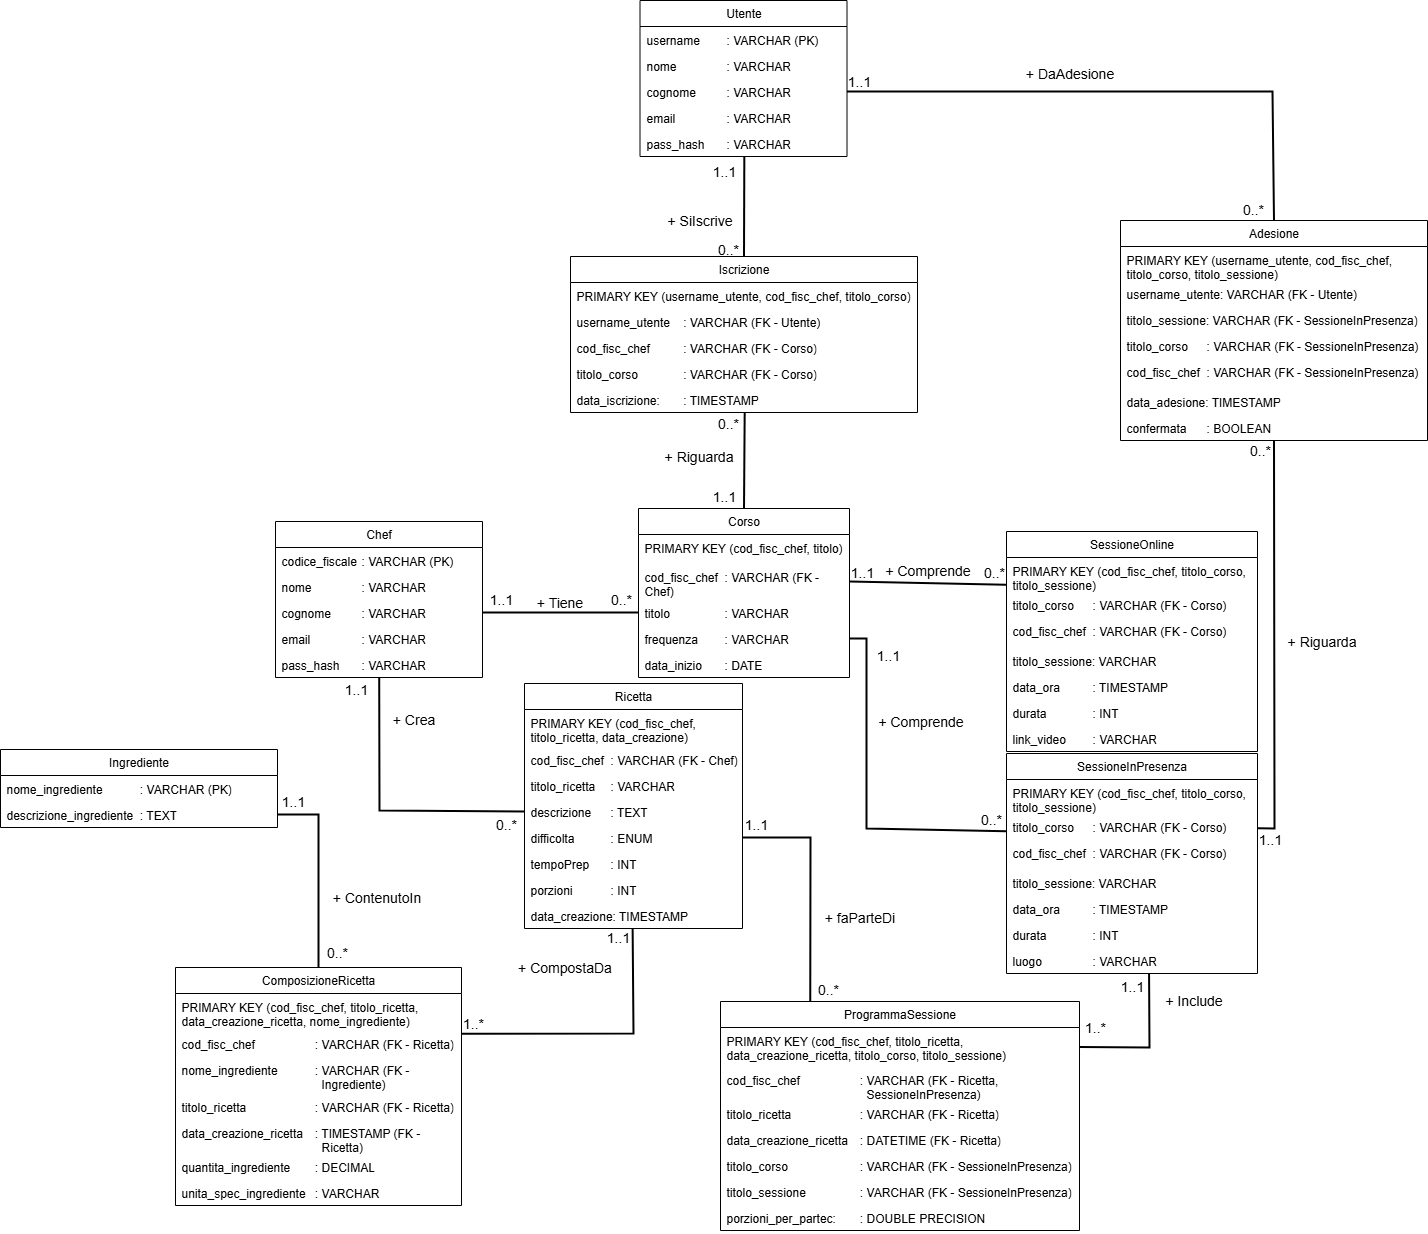
\includegraphics[width=0.9\linewidth]{pics/DiagrammaUML-Ristrutturato.png}
        \caption{\label{fig:DiagrammaUMLRistrutturato}Diagramma Ristrutturato UML}
    \end{figure}

    \subsection{Procedure effettuate sul diagramma}
        \subsubsection{Conversione di tutte le classi in tabelle} La prima cosa fatta è stata adattare il diagramma in maniera tale che fosse compatibile con ciò che ci interessa, la costruzione della base di dati. Per questo motivo sono state convertite tutte le classi in tabelle con attributi SQL veri e propri.
    
        \subsubsection{Scelta di attributi coerenti con il linguaggio} Sono stati selezionati, invece che delle vaghe "String", come nel diagramma precedente, degli attributi coerenti con SQL: ogni tipo è stato selezionato in base a quale rispecchiasse meglio la natura del dato del caso.
    
        \subsubsection{Gestione delle relazioni 1:N} Le relazioni 1:N come \texttt{Chef-Corso} sono state gestite implementando delle chiavi esterne (FK).
    
        \subsubsection{Eliminazione della generalizzazione} Le generalizzazioni EER/UML sono costrutti non direttamente disponibili nel modello relazionale e quindi vanno sostituite con altre tecniche.\\[0.2cm]
        Per la gerarchia \texttt{Sessione \{SessioneOnline, SessioneInPresenza\}} si è scelta la strategia Concrete Table Inheritance: la superclasse \texttt{Sessione} è stata rimossa e gli attributi comuni sono stati duplicati nelle due tabelle concrete \texttt{SessioneOnline} e \texttt{SessioneInPresenza}. Questa scelta rende compatibile il diagramma con il linguaggio SQL e distingue i due tipi di sessioni, a costo della duplicazione controllata degli attributi comuni.
    
        \subsubsection{Scelta degli identificatori principali}
        Per ogni classe è stato definito un identificatore univoco (chiave primaria). Per alcune classi l'identificatore era singolo e naturale, per altre è composto da due o più attributi, sia appartenenti alla classe specifica, sia chiavi esterne che riconducono ad altre classi.
    
        \subsubsection{Creazione relazione Ricetta-Chef}
        Si è creata una nuova relazione "Crea" tra Ricetta e Chef, dato l'utilizzo in chiave primaria della chiave esterna del codice fiscale dello Chef da parte della classe Ricetta.
    
        \bigskip
        In conclusione, la ristrutturazione ha prodotto uno schema UML ristrutturato coerente con l'implementazione relazionale in MySQL: tutte le associazioni sono espresse tramite FK o tabelle ponte, le generalizzazioni sono state risolte tramite tabelle concrete e le chiavi primarie/esterne sono state definite in modo da preservare l'integrità referenziale e consentire operazioni di calcolo in modo efficiente.

    \newpage
    
    \subsection{Dizionario delle classi, delle associazioni, e dei vincoli}
    In questa sezione creeremo il dizionario delle classi: uno strumento utile a rendere chiaro, in maniera più verbale/testuale rispetto ai diagrammi visti finora, le classi della nostra base di dati, gli attributi che hanno, e le relazioni. Qui definiremo anche, per ogni classe, i vincoli di cui i loro attributi godono.

    \subsubsection*{Classe Utente}
        \textbf{Descrizione:} Rappresenta un utente generico del sistema.
        
        {
        \vspace{1em}
        \renewcommand{\arraystretch}{1.3}
        \begin{tabular}{|l|l|l|l|}
        \hline
        \textbf{Attributo} & \textbf{Tipo} & \textbf{Descrizione} & \textbf{Vincoli} \\
        \hline
        username & VARCHAR      & Identificativo univoco utente & PK \\
        nome     & VARCHAR      & Nome dell'utente & Not null \\
        cognome  & VARCHAR      & Cognome dell'utente & Not null \\
        email    & VARCHAR      & Indirizzo email & Unique Not null \\
        pass\_hash & VARCHAR      & Credenziali di accesso & Not null \\
        \hline
        \end{tabular}\\[0.5em]
        }

        \noindent\textbf{Relazioni:}  
        - 0..* con \textit{Iscrizione}  
        - 0..* con \textit{Adesione}

    \noindent\rule{\textwidth}{0.1pt}

    \subsubsection*{Classe Chef}
        \textbf{Descrizione:} Rappresenta un cuoco responsabile della preparazione delle ricette e della conduzione delle sessioni pratiche.
        
        {
        \vspace{1em}
        \renewcommand{\arraystretch}{1.3}
        \begin{tabular}{|l|l|l|l|}
        \hline
        \textbf{Attributo} & \textbf{Tipo} & \textbf{Descrizione} & \textbf{Vincoli} \\
        \hline
        codice\_fiscale & VARCHAR      & Identificativo univoco cuoco & PK \\
        nome            & VARCHAR      & Nome del cuoco & Not null \\
        cognome         & VARCHAR      & Cognome del cuoco & Not null \\
        email           & VARCHAR      & Indirizzo email & Unique Not null \\
        pass\_hash      & VARCHAR      & Credenziali di accesso & Not null \\
        \hline
        \end{tabular}\\[0.5em]
        }
        
        \noindent\textbf{Relazioni:}  
        - 0..* con \textit{Ricetta} (uno Chef può creare più ricette)  
        - 0..* con \textit{Corso} (uno Chef può creare più corsi)

    \newpage

    \subsubsection*{Classe Corso}
        \textbf{Descrizione:} Rappresenta un corso formativo creato da un determinato chef e composto da più sessioni.
        
        {
        \vspace{1em}
        \renewcommand{\arraystretch}{1.3}
        \begin{tabularx}{\textwidth}{|l|l|X|l|}
            \hline
            \textbf{Attributo} & \textbf{Tipo} & \textbf{Descrizione} & \textbf{Vincoli} \\
            \hline
            cod\_fisc\_chef & VARCHAR      & Codice fiscale dello chef che tiene il corso & FK, Not null \\
            titolo          & VARCHAR      & Titolo identificativo del corso & Not null \\
            frequenza       & VARCHAR      & Frequenza delle lezioni (es. settimanale) & \\
            data\_inizio    & DATE         & Data di inizio del corso & Not null \\
            \hline
            \end{tabularx}\\[0.5em]
        }
        
        \noindent\textbf{Chiave primaria composta:} (cod\_fisc\_chef, titolo)\\[0.1em]  
        
        \noindent\textbf{Relazioni:}  
        - 1..1 con \textit{Chef} (ogni corso è tenuto da un singolo chef)  
        - 0..* con \textit{SessioneOnline} e \textit{SessioneInPresenza} (un corso comprende più sessioni)  
        - 0..* con \textit{Iscrizione} (gli utenti possono iscriversi a un corso)

    \noindent\rule{\textwidth}{0.1pt}

    \subsubsection*{Classe Ricetta}
        \textbf{Descrizione:} Rappresenta una ricetta creata da uno chef e legata a uno o più corsi tramite i programmi delle sessioni.
        
        {
        \vspace{1em}
        \renewcommand{\arraystretch}{1.3}
        \begin{tabularx}{\textwidth}{|l|l|X|l|}
        \hline
        \textbf{Attributo} & \textbf{Tipo} & \textbf{Descrizione} & \textbf{Vincoli} \\
        \hline
        cod\_fisc\_chef    & VARCHAR       & Codice fiscale chef & FK, Not null \\
        titolo\_ricetta    & VARCHAR       & Titolo della ricetta & Not null \\
        data\_creazione    & TIMESTAMP     & Data di creazione ricetta & Not null \\
        descrizione        & TEXT          & descrizione della ricetta & \\
        difficolta         & ENUM          & Livello di difficoltà & \\
        tempoPrep          & INT           & Tempo di preparazione & \\
        porzioni           & INT           & Numero di porzioni & \\
        \hline
        \end{tabularx}\\[0.5em]
        }
        
        \noindent\textbf{Chiave primaria composta:} (cod\_fisc\_chef, titolo\_ricetta, data\_creazione)\\[0.1em] 
        
        \noindent\textbf{Relazioni:}  
        - 1..1 con \textit{Chef} (ogni ricetta è creata da un solo chef)  
        - 1..* con \textit{ComposizioneRicetta} (ingredienti che compongono la ricetta)  
        - 0..* con \textit{ProgrammaSessione} (la ricetta può essere inclusa in più sessioni)

    \newpage

    \subsubsection*{Classe ComposizioneRicetta}
        \textbf{Descrizione:} Rappresenta l’associazione tra una ricetta e i suoi ingredienti, specificando quantità e unità di misura.
        
        {
        \vspace{1em}
        \renewcommand{\arraystretch}{1.3}
        \begin{tabularx}{\textwidth}{|l|l|X|l|}
        \hline
        \textbf{Attributo} & \textbf{Tipo} & \textbf{Descrizione} & \textbf{Vincoli} \\
        \hline
        cod\_fisc\_chef       & VARCHAR        & Codice chef & FK, Not null \\
        titolo\_ricetta       & VARCHAR        & Titolo della ricetta & FK, Not null \\
        data\_creazione\_ric  & TIMESTAMP      & Data di creazione ricetta & FK, Not null \\
        nome\_ingrediente     & VARCHAR        & Nome dell’ingrediente & FK, Not null \\
        quantita              & DECIMAL        & Quantità dell’ingrediente & \\
        unita\_spec           & VARCHAR        & Unità di misura (es. g, ml, cucchiai) & \\
        \hline
        \end{tabularx}\\[0.5em]
        }
        
        \noindent\textbf{Chiave primaria composta:} (cod\_fisc\_chef, titolo\_ricetta, data\_creazione\_ricetta, nome\_ingrediente)\\[0.1em]  
        
        \noindent\textbf{Relazioni:}  
        - 1..1 con \textit{Ricetta} (ogni composizione appartiene a una ricetta)  
        - 1..1 con \textit{Ingrediente} (ogni composizione fa riferimento a un ingrediente)

    \noindent\rule{\textwidth}{0.1pt}

    \subsubsection*{Classe Ingrediente}
        \textbf{Descrizione:} Rappresenta un singolo ingrediente utilizzabile nelle ricette, con relativa descrizione.
        
        {
        \vspace{1em}
        \renewcommand{\arraystretch}{1.3}
        \begin{tabularx}{\textwidth}{|l|l|X|l|}
        \hline
        \textbf{Attributo} & \textbf{Tipo} & \textbf{Descrizione} & \textbf{Vincoli} \\
        \hline
        nome\_ingrediente      & VARCHAR       & Nome univoco dell’ingrediente & PK \\
        descrizione\_ingrediente & TEXT        & Descrizione dettagliata dell’ingrediente & \\
        \hline
        \end{tabularx}\\[0.5em]
        }
        
        \noindent\textbf{Relazioni:}  
        - 0..* con \textit{ComposizioneRicetta} (un ingrediente può comparire in più ricette)

    \newpage

    \subsubsection*{Classe ProgrammaSessione}
        \textbf{Descrizione:} Rappresenta l’associazione tra una sessione di un corso e le ricette trattate al suo interno, specificando le porzioni per partecipante.
        
        {
        \vspace{1em}
        \renewcommand{\arraystretch}{1.3}
        \begin{tabularx}{\textwidth}{|l|l|X|l|}
        \hline
        \textbf{Attributo} & \textbf{Tipo} & \textbf{Descrizione} & \textbf{Vincoli} \\
        \hline
        cod\_fisc\_chef       & VARCHAR      & Codice fiscale chef & FK, Not null \\
        titolo\_ricetta       & VARCHAR      & Titolo della ricetta & FK, Not null \\
        data\_creazione\_ricetta & TIMESTAMP & Data di creazione ricetta & FK, Not null \\
        titolo\_corso         & VARCHAR      & Titolo del corso & FK, Not null \\
        titolo\_sessione      & VARCHAR      & Titolo della sessione & FK, Not null \\
        porzioni\_per\_partec & DOUBLE PRECISION & Numero di porzioni per ogni partecipante & \\
        \hline
        \end{tabularx}\\[0.5em]
        }
        
        \noindent\textbf{Chiave primaria composta:}  
        (cod\_fisc\_chef, titolo\_ricetta, data\_creazione\_ricetta, titolo\_corso, titolo\_sessione)\\[0.1em]
        
        \noindent\textbf{Relazioni:}  
        - 1..1 con \textit{Ricetta} (ogni record associa una ricetta a una sessione)  
        - 1..1 con \textit{SessioneInPresenza} (ogni record appartiene a una specifica sessione in presenza)

    \noindent\rule{\textwidth}{0.1pt}

    \subsubsection*{Classe SessioneInPresenza}
        \textbf{Descrizione:} Rappresenta una singola sessione di un corso svolta in presenza, con indicazione di data, orario e luogo.
        
        {
        \vspace{1em}
        \renewcommand{\arraystretch}{1.3}
        \begin{tabularx}{\textwidth}{|l|l|X|l|}
        \hline
        \textbf{Attributo} & \textbf{Tipo} & \textbf{Descrizione} & \textbf{Vincoli} \\
        \hline
        titolo\_corso    & VARCHAR      & Titolo del corso & FK, Not null \\
        titolo\_sessione & VARCHAR      & Titolo della sessione & Not null \\
        cod\_fisc\_chef  & VARCHAR      & Identificativo Chef & FK, Not null \\
        data\_ora        & TIMESTAMP    & Data e orario sessione & Not null \\
        durata           & INT          & Durata sessione & \\
        luogo            & VARCHAR      & Luogo della sessione & \\
        \hline
        \end{tabularx}\\[0.5em]
        }
        
        \noindent\textbf{Chiave primaria composta:} (cod\_fisc\_chef, titolo\_corso, titolo\_sessione)\\[0.1em]
        
        \noindent\textbf{Relazioni:}  
        - 1..1 con \textit{Corso} (ogni sessione appartiene a un corso)  
        - 1..* con \textit{ProgrammaSessione} (una sessione può includere più ricette)  
        - 0..* con \textit{Adesione} (una sessione può avere più partecipanti iscritti)

    \noindent\rule{\textwidth}{0.1pt}

    \subsubsection*{Classe SessioneOnline}
        \textbf{Descrizione:} Rappresenta una sessione di corso svolta online, con indicazione della piattaforma e delle credenziali di accesso.
        
        {
        \vspace{1em}
        \renewcommand{\arraystretch}{1.3}
        \begin{tabularx}{\textwidth}{|l|l|X|l|}
        \hline
        \textbf{Attributo} & \textbf{Tipo} & \textbf{Descrizione} & \textbf{Vincoli} \\
        \hline
        cod\_fisc\_chef  & VARCHAR      & Identificativo Chef & FK, Not null \\
        titolo\_corso    & VARCHAR      & Titolo del corso & FK, Not null \\
        titolo\_sessione & VARCHAR      & Titolo della sessione & Not null \\
        data\_ora        & TIMESTAMP    & Data e orario della sessione & Not null \\
        durata           & INT          & Durata sessione & \\
        link\_video      & VARCHAR      & Link del video sessione & \\
        \hline
        \end{tabularx}\\[0.5em]
        }
        
        \noindent\textbf{Chiave primaria composta:} (cod\_fisc\_chef, titolo\_corso, titolo\_sessione)\\[0.1em]
        
        \noindent\textbf{Relazioni:}  
        - 1..1 con \textit{Corso} (ogni sessione online appartiene a un corso)
        
    \noindent\rule{\textwidth}{0.1pt}

    \subsubsection*{Classe Iscrizione}
        \textbf{Descrizione:} Rappresenta l'iscrizione di un utente a un corso, con la relativa data di iscrizione.
        
        {
        \vspace{1em}
        \renewcommand{\arraystretch}{1.3}
        \begin{tabularx}{\textwidth}{|l|l|X|l|}
        \hline
        \textbf{Attributo} & \textbf{Tipo} & \textbf{Descrizione} & \textbf{Vincoli} \\
        \hline
        username\_utente    & VARCHAR         & Identificativo dell'utente iscritto & FK, Not null \\
        cod\_fisc\_chef & VARCHAR     & Codice fiscale dello chef & FK, Not null \\
        titolo\_corso & VARCHAR       & Titolo del corso a cui ci si iscrive & FK, Not null \\
        data\_iscrizione & TIMESTAMP  & Data in cui l'utente si è iscritto & Not null \\
        \hline
        \end{tabularx}\\[0.5em]
        }
        
        \noindent\textbf{Chiave primaria composta:} (cod\_fisc\_chef, username\_utente, titolo\_corso)\\[0.1em]
        
        \noindent\textbf{Relazioni:}  
        - 1..1 con \textit{Utente} (ogni iscrizione è riferita a un utente)  
        - 1..1 con \textit{Corso} (ogni iscrizione è riferita a un corso)

    \newpage

    \subsubsection*{Classe Adesione}
        \textbf{Descrizione:} Rappresenta la partecipazione effettiva di un utente a una specifica sessione (in presenza o online) di un corso a cui è iscritto.
        
        {
        \vspace{1em}
        \renewcommand{\arraystretch}{1.3}
        \begin{tabularx}{\textwidth}{|l|l|X|l|}
        \hline
        \textbf{Attributo} & \textbf{Tipo} & \textbf{Descrizione} & \textbf{Vincoli} \\
        \hline
        username\_utente & VARCHAR  & Identificativo dell'utente & FK, Not null \\
        titolo\_corso   & VARCHAR  & Titolo del corso della sessione & FK, Not null \\
        cod\_fisc\_chef & VARCHAR  & Codice fiscale dello chef & FK, Not null \\
        titolo\_sessione & VARCHAR  & Titolo della sessione & FK, Not null \\
        data\_adesione   & TIMESTAMP     & Data e orario dell'adesione & Not null \\
        confermata       & BOOLEAN      & Conferma dell'adesione & \\
        \hline
        \end{tabularx}\\[0.5em]
        }
        
        \noindent\textbf{Chiave primaria composta:} (username\_utente, titolo\_corso, cod\_fisc\_chef, titolo\_sessione)\\[0.2em]
        
        \noindent\textbf{Relazioni:}  
        - 1..1 con \textit{Utente} (ogni adesione è riferita a un utente)  
        - 1..1 con \textit{SessioneInPresenza} / \textit{SessioneOnline} (ogni adesione è riferita a una specifica sessione di corso)

    \newpage

\section{Schema Fisico}
    Entriamo quindi nelle ultime fasi della creazione di questo database, lo \textbf{schema fisico}. Per schema fisico intendiamo la base di dati completamente implementata in linguaggio SQL utilizzando un DBMS di nostra scelta. Inoltre, lo schema fisico comprende anche i vari \textit{trigger}, \textit{procedure}, e il \textit{popolamento del database} stesso.\\[0.2cm]
    In questa sezione andremo quindi ad analizzare ogni fase di questo processo, dalla scelta del DBMS, la scrittura della base di dati, fino ad arrivare al suo popolamento e, di conseguenza, completamento, in modo da renderlo perfettamente compatibile e comunicante con l'applicativo Java. In questa maniera arriveremo a completare il progetto.

    \subsection{Scelta del DBMS e installazione}
    La scelta del DBMS da utilizzare per questa base di dati è ricaduta su \textbf{PostgreSQL}, la motivazione è da trovarsi nella sua semplicità e fedeltà agli standard SQL, soprattutto quando combinato con Java tramite driver JDBC.\\[0.2cm]
    In questo contesto ci limiteremo ad installare PostgreSQL senza andare poi ad utilizzare programmi come pgAdmin per gestirlo ed utilizzarlo, dato che per progettare tutta la base di dati utilizzeremo un mix tra \textit{terminale CMD (Windows)}, e \textit{Visual Studio Code}.
    \begin{itemize}
        \item Scarichiamo e installiamo PostgreSQL dal sito ufficiale.
        \item Scegliamo una password per il profilo utente che andremo ad utilizzare (postgres).
        \item Scegliamo la porta (default: 5432).
    \end{itemize}

    \subsection{Creazione e connessione al database}
    Adesso è il momento di creare il vero e proprio database all'interno del DBMS. Lo facciamo molto semplicemente aprendo il CMD di Windows, collegandoci al server di PostgreSQL tramite path e credenziali, e utilizzando quindi SQL per creare la base di dati (possiamo conservare la creazione del db, tabelle, popolamento e molto altro in file ".sql" appositi):
    \begin{lstlisting}[style=sqlstyle]
    -- ====================================================
    -- File: create_database.sql
    -- Descrizione: Crea il database del progetto
    -- Autore: Salvatore De Pasquale
    -- ====================================================
    
    -- Crea il database
    CREATE DATABASE UninaFoodLab;
    \end{lstlisting}
    Fatto ciò, ci connetteremo al database. Possiamo farlo tramite comando "\textbackslash c UninaFoodLab".

    \newpage
    \subsection{Creazione dello schema del database}
    Andremo ora a creare lo schema della nostra base di dati, ossia tutte le classi, gli attributi, eventuali ENUM, e tutto ciò che riguarda la struttura del db. In sostanza questo è il momento di andare a definire in SQL tutto ciò che abbiamo progettato fino ad ora.
    \begin{lstlisting}[style=sqlstyle]
    -- ====================================================
    -- File: create_tables.sql
    -- Descrizione: Definisce tutta la struttura della base di dati
    -- Autore: Salvatore De Pasquale
    -- ====================================================
    
    BEGIN;
    \end{lstlisting}
    Il file inizia così, con una transazione. Ciò ci garantisce coerenza durante la creazione della base di dati, poiché una transazione definisce una serie di azioni che verranno eseguite \textbf{tutte}, oppure \textbf{nessuna}.\\[0.2cm]
    Andremo adesso a definire, nello stesso file, tutto ciò che ci serve.
        \subsubsection{Definizione di Chef}
        \begin{lstlisting}[style=sqlstyle]
        -- Definizione tabella Chef
        
        CREATE TABLE Chef(
            codice_fiscale VARCHAR (16) PRIMARY KEY,
            nome VARCHAR(50) NOT NULL,
            cognome VARCHAR(50) NOT NULL,
            email VARCHAR(254) UNIQUE NOT NULL,
            pass_hash VARCHAR(50) NOT NULL
        );
        \end{lstlisting}
        \subsubsection{Definizione di Corso}
        \begin{lstlisting}[style=sqlstyle]
        -- Definizione tabella Corso
        
        CREATE TABLE Corso(
            cod_fisc_chef VARCHAR(16) NOT NULL REFERENCES Chef(codice_fiscale) ON DELETE CASCADE,
            titolo VARCHAR(50) NOT NULL,
            frequenza VARCHAR(50),
            data_inizio DATE NOT NULL,
            PRIMARY KEY(cod_fisc_chef, titolo)
        );
        \end{lstlisting}
        \newpage
        \subsubsection{Definizione dell'ENUM stadi\_difficolta}
        \begin{lstlisting}[style=sqlstyle]
        -- Creiamo l'ENUM per la tabella Ricetta
        
        CREATE TYPE stadi_difficolta AS ENUM ('facile', 'medio', 'difficile');
        \end{lstlisting}
        \subsubsection{Definizione di Ricetta}
        \begin{lstlisting}[style=sqlstyle]
        -- Definizione tabella Ricetta
        
        CREATE TABLE Ricetta(
            cod_fisc_chef VARCHAR(16) NOT NULL REFERENCES Chef(codice_fiscale) ON DELETE CASCADE,
            titolo_ricetta VARCHAR(50) NOT NULL,
            descrizione TEXT,
            difficolta stadi_difficolta,
            tempo_prep INT,
            porzioni INT,
            data_creazione TIMESTAMP NOT NULL DEFAULT CURRENT_TIMESTAMP,
            PRIMARY KEY (cod_fisc_chef, titolo_ricetta, data_creazione)
        );
        \end{lstlisting}
        \subsubsection{Definizione di Utente}
        \begin{lstlisting}[style=sqlstyle]
        -- Definizione tabella Utente
        
        CREATE TABLE Utente(
            username VARCHAR(30) PRIMARY KEY,
            nome VARCHAR(50) NOT NULL,
            cognome VARCHAR(50) NOT NULL,
            email VARCHAR(254) UNIQUE NOT NULL,
            pass_hash VARCHAR(50) NOT NULL
        );
        \end{lstlisting}
        \subsubsection{Definizione di Ingrediente}
        \begin{lstlisting}[style=sqlstyle]
        -- Definizione tabella Ingrediente
        
        CREATE TABLE Ingrediente(
            nome_ingrediente VARCHAR(25) PRIMARY KEY,
            descrizione_ingrediente TEXT
        );
        \end{lstlisting}
        \newpage
        \subsubsection{Definizione di SessioneOnline}
        \begin{lstlisting}[style=sqlstyle]
        -- Definizione SessioneOnline
        
        CREATE TABLE SessioneOnline (
            cod_fisc_chef VARCHAR(16) NOT NULL,
            titolo_corso VARCHAR(50) NOT NULL,
            titolo_sessione VARCHAR(50) NOT NULL,
            data_ora TIMESTAMP NOT NULL,
            durata INT,
            link_video VARCHAR(2083),
            PRIMARY KEY (cod_fisc_chef, titolo_corso, titolo_sessione),
            FOREIGN KEY (cod_fisc_chef, titolo_corso) REFERENCES Corso(cod_fisc_chef, titolo) ON DELETE CASCADE
        );
        \end{lstlisting}
        \subsubsection{Definizione di SessioneInPresenza}
        \begin{lstlisting}[style=sqlstyle]
        -- Definizione SessioneInPresenza
        
        CREATE TABLE SessioneInPresenza(
            cod_fisc_chef VARCHAR(16) NOT NULL,
            titolo_corso VARCHAR(50) NOT NULL,
            titolo_sessione VARCHAR(50) NOT NULL,
            data_ora TIMESTAMP NOT NULL,
            durata INT,
            luogo VARCHAR(100),
            posti_totali INT,
            posti_disponibili INT,
            PRIMARY KEY (cod_fisc_chef, titolo_corso, titolo_sessione),
            FOREIGN KEY (cod_fisc_chef, titolo_corso) REFERENCES Corso(cod_fisc_chef, titolo) ON DELETE CASCADE
        );
        \end{lstlisting}
        \subsubsection{Definizione di Iscrizione}
        \begin{lstlisting}[style=sqlstyle]
        -- Definizione Iscrizione
        
        CREATE TABLE Iscrizione(
            username_utente VARCHAR(30) NOT NULL,
            cod_fisc_chef VARCHAR(16) NOT NULL,
            titolo_corso VARCHAR(50) NOT NULL,
            data_iscrizione TIMESTAMP NOT NULL DEFAULT CURRENT_TIMESTAMP,
            PRIMARY KEY (username_utente, cod_fisc_chef, titolo_corso),
            FOREIGN KEY (cod_fisc_chef, titolo_corso) REFERENCES Corso(cod_fisc_chef, titolo) ON DELETE CASCADE,
            FOREIGN KEY (username_utente) REFERENCES Utente(username) ON DELETE CASCADE
        );
        \end{lstlisting}
        \subsubsection{Definizione di Adesione}
        \begin{lstlisting}[style=sqlstyle]
        -- Definizione Adesione
        
        CREATE TABLE Adesione(
            username_utente VARCHAR(30) NOT NULL,
            titolo_corso VARCHAR(50) NOT NULL,
            titolo_sessione VARCHAR(50) NOT NULL,
            cod_fisc_chef VARCHAR(16) NOT NULL,
            data_adesione TIMESTAMP NOT NULL DEFAULT CURRENT_TIMESTAMP,
            confermata BOOLEAN,
            PRIMARY KEY (username_utente, cod_fisc_chef, titolo_corso, titolo_sessione),
            FOREIGN KEY (username_utente) REFERENCES Utente(username) ON DELETE CASCADE,
            FOREIGN KEY (cod_fisc_chef, titolo_corso, titolo_sessione) REFERENCES SessioneInPresenza(cod_fisc_chef, titolo_corso, titolo_sessione) ON DELETE CASCADE
        );
        \end{lstlisting}
        \subsubsection{Definizione di ProgrammaSessione}
        \begin{lstlisting}[style=sqlstyle]
        -- Definizione ProgrammaSessione
        
        CREATE TABLE ProgrammaSessione(
            cod_fisc_chef VARCHAR(16) NOT NULL,
            titolo_ricetta VARCHAR(50) NOT NULL,
            data_creazione_ricetta TIMESTAMP NOT NULL,
            titolo_corso VARCHAR(50) NOT NULL,
            titolo_sessione VARCHAR(50) NOT NULL,
            porzioni_per_partec DOUBLE PRECISION,
            PRIMARY KEY (cod_fisc_chef, titolo_ricetta, data_creazione_ricetta, titolo_corso, titolo_sessione),
            FOREIGN KEY (cod_fisc_chef, titolo_ricetta, data_creazione_ricetta) REFERENCES Ricetta(cod_fisc_chef, titolo_ricetta, data_creazione) ON DELETE CASCADE,
            FOREIGN KEY (cod_fisc_chef, titolo_corso, titolo_sessione) REFERENCES SessioneInPresenza(cod_fisc_chef, titolo_corso, titolo_sessione) ON DELETE CASCADE
        );
        \end{lstlisting}
        \newpage
        \subsubsection{Definizione di ComposizioneRicetta}
        \begin{lstlisting}[style=sqlstyle]
        -- Definizione di ComposizioneRicetta
        
        CREATE TABLE ComposizioneRicetta(
            cod_fisc_chef VARCHAR(16) NOT NULL,
            nome_ingrediente VARCHAR(25) NOT NULL,
            titolo_ricetta VARCHAR(50) NOT NULL,
            data_creazione_ricetta TIMESTAMP NOT NULL,
            quantita_ingrediente DECIMAL(6,2),
            unita_spec_ingrediente VARCHAR(10),
            PRIMARY KEY (cod_fisc_chef, titolo_ricetta, data_creazione_ricetta, nome_ingrediente),
            FOREIGN KEY (cod_fisc_chef, titolo_ricetta, data_creazione_ricetta) REFERENCES Ricetta(cod_fisc_chef, titolo_ricetta, data_creazione) ON DELETE CASCADE,
            FOREIGN KEY (nome_ingrediente) REFERENCES Ingrediente(nome_ingrediente) ON DELETE RESTRICT
        );
        \end{lstlisting}
        Chiudiamo ora il file con:
        \begin{lstlisting}[style=sqlstyle]
        
        COMMIT;
        \end{lstlisting}
        In modo da completare la preparazione della transazione.

    \subsection{Popolamento del database}
    Andremo adesso a popolare il database con dei dati che utilizzeremo per testare l'applicativo e le varie funzionalità che SQL ci fornisce per manipolare i dati.\\[0.2cm]
    Iniziamo il file "populate\_database.sql" così:
    \begin{lstlisting}[style=sqlstyle]
    -- ====================================================
    -- File: populate_database.sql
    -- Descrizione: Popola il database UninaFoodLab con dati
    -- Autore: Salvatore De Pasquale
    -- ====================================================
    
    BEGIN;
    \end{lstlisting}
    \newpage
        \subsubsection{Inserimento Chef}
        \begin{lstlisting}[style=sqlstyle]
        - -------------------------
        -- TABELLA CHEF
        -- -------------------------
        INSERT INTO Chef (codice_fiscale, nome, cognome, email, pass_hash)
        VALUES 
        ('RSSMRA85M01H501U', 'Mario', 'Rossi', 'mario.rossi@example.com', 'hashpassword123'),
        ('BNCLRA90L45F839K', 'Lara', 'Bianchi', 'lara.bianchi@example.com', 'hashpassword456');
        \end{lstlisting}
        \subsubsection{Inserimento Corso}
        \begin{lstlisting}[style=sqlstyle]
        -- -------------------------
        -- TABELLA CORSO
        -- -------------------------
        INSERT INTO Corso (cod_fisc_chef, titolo, frequenza, data_inizio)
        VALUES 
        ('RSSMRA85M01H501U', 'Cucina Italiana', 'settimanale', '2025-10-20'),
        ('BNCLRA90L45F839K', 'Dolci al Cucchiaio', 'mensile', '2025-11-05');
        \end{lstlisting}
        \subsubsection{Inserimento Utente}
        \begin{lstlisting}[style=sqlstyle]
        -- -------------------------
        -- TABELLA UTENTE
        -- -------------------------
        INSERT INTO Utente (username, nome, cognome, email, pass_hash)
        VALUES
        ('giulia123', 'Giulia', 'Bianchi', 'giulia.bianchi@example.com', 'hashpass456'),
        ('andrea88', 'Andrea', 'Verdi', 'andrea.verdi@example.com', 'hashpass789');
        \end{lstlisting}
        \subsubsection{Inserimento Ingrediente}
        \begin{lstlisting}[style=sqlstyle]
        -- -------------------------
        -- TABELLA INGREDIENTE
        -- -------------------------
        INSERT INTO Ingrediente (nome_ingrediente, descrizione_ingrediente)
        VALUES
        ('Pomodoro', 'Pomodoro fresco maturo'),
        ('Basilico', 'Foglie di basilico fresco'),
        ('Zucchero', 'Zucchero semolato'),
        ('Latte', 'Latte intero fresco');
        \end{lstlisting}
        \subsubsection{Inserimento Ricetta}
        \begin{lstlisting}[style=sqlstyle]
        -- -------------------------
        -- TABELLA RICETTA
        -- -------------------------
        INSERT INTO Ricetta (cod_fisc_chef, titolo_ricetta, descrizione, difficolta, tempo_prep, porzioni, data_creazione)
        VALUES
        ('RSSMRA85M01H501U', 'Pasta al Pomodoro', 'Ricetta tradizionale italiana', 'facile', 30, 4, '2025-10-15 18:00:00'),
        ('BNCLRA90L45F839K', 'Panna Cotta', 'Dolce al cucchiaio con panna e zucchero', 'medio', 45, 6, '2025-10-14 10:30:00');
        \end{lstlisting}
        \subsubsection{Inserimento SessioneInPresenza}
        \begin{lstlisting}[style=sqlstyle]
        -- -------------------------
        -- TABELLA SESSIONE IN PRESENZA
        -- -------------------------
        INSERT INTO SessioneInPresenza (cod_fisc_chef, titolo_corso, titolo_sessione, data_ora, durata, luogo)
        VALUES
        ('RSSMRA85M01H501U', 'Cucina Italiana', 'Lezione 1', '2025-10-21 15:30:00', 120, 'Napoli'),
        ('BNCLRA90L45F839K', 'Dolci al Cucchiaio', 'Lezione 1', '2025-11-07 17:00:00', 90, 'Milano');
        \end{lstlisting}
        \subsubsection{Inserimento SessioneOnline}
        \begin{lstlisting}[style=sqlstyle]
        -- -------------------------
        -- TABELLA SESSIONE ONLINE
        -- -------------------------
        INSERT INTO SessioneOnline (cod_fisc_chef, titolo_corso, titolo_sessione, data_ora, durata, link_video)
        VALUES
        ('RSSMRA85M01H501U', 'Cucina Italiana', 'Lezione Online 1', '2025-10-23 18:00:00', 90, 'https://zoom.example.com/mario'),
        ('BNCLRA90L45F839K', 'Dolci al Cucchiaio', 'Lezione Online 1', '2025-11-09 20:30:00', 60, 'https://zoom.example.com/lara');
        \end{lstlisting}
        \newpage
        \subsubsection{Inserimento Iscrizione}
        \begin{lstlisting}[style=sqlstyle]
        -- -------------------------
        -- TABELLA ISCRIZIONE
        -- -------------------------
        INSERT INTO Iscrizione (username_utente, cod_fisc_chef, titolo_corso, data_iscrizione)
        VALUES
        ('giulia123', 'RSSMRA85M01H501U', 'Cucina Italiana', '2025-10-15 18:10:00'),
        ('andrea88', 'BNCLRA90L45F839K', 'Dolci al Cucchiaio', '2025-10-16 09:45:00');
        \end{lstlisting}
        \subsubsection{Inserimento Adesione}
        \begin{lstlisting}[style=sqlstyle]
        -- -------------------------
        -- TABELLA ADESIONE
        -- -------------------------
        INSERT INTO Adesione (username_utente, titolo_corso, titolo_sessione, cod_fisc_chef, data_adesione, confermata)
        VALUES
        ('giulia123', 'Cucina Italiana', 'Lezione 1', 'RSSMRA85M01H501U', '2025-10-17 10:00:00', TRUE),
        ('andrea88', 'Dolci al Cucchiaio', 'Lezione 1', 'BNCLRA90L45F839K', '2025-10-18 11:00:00', FALSE);
        \end{lstlisting}
        \subsubsection{Inserimento ComposizioneRicetta}
        \begin{lstlisting}[style=sqlstyle]
        -- -------------------------
        -- TABELLA COMPOSIZIONE RICETTA
        -- -------------------------
        INSERT INTO ComposizioneRicetta (cod_fisc_chef, nome_ingrediente, titolo_ricetta, data_creazione_ricetta, quantita_ingrediente, unita_spec_ingrediente)
        VALUES
        ('RSSMRA85M01H501U', 'Pomodoro', 'Pasta al Pomodoro', '2025-10-15 18:00:00', 200.0, 'g'),
        ('RSSMRA85M01H501U', 'Basilico', 'Pasta al Pomodoro', '2025-10-15 18:00:00', 5.0, 'foglie'),
        ('BNCLRA90L45F839K', 'Latte', 'Panna Cotta', '2025-10-14 10:30:00', 500.0, 'ml'),
        ('BNCLRA90L45F839K', 'Zucchero', 'Panna Cotta', '2025-10-14 10:30:00', 100.0, 'g');
        \end{lstlisting}
        \newpage
        \subsubsection{Inserimento ProgrammaSessione}
        \begin{lstlisting}[style=sqlstyle]
        -- -------------------------
        -- TABELLA PROGRAMMA SESSIONE
        -- -------------------------
        INSERT INTO ProgrammaSessione (cod_fisc_chef, titolo_ricetta, data_creazione_ricetta, titolo_corso, titolo_sessione, porzioni_per_partec)
        VALUES
        ('RSSMRA85M01H501U', 'Pasta al Pomodoro', '2025-10-15 18:00:00', 'Cucina Italiana', 'Lezione 1', 2.0),
        ('BNCLRA90L45F839K', 'Panna Cotta', '2025-10-14 10:30:00', 'Dolci al Cucchiaio', 'Lezione 1', 1.5);
        
        COMMIT;
        \end{lstlisting}

    \subsection{Creazione Trigger e Funzioni}
    Adesso andremo a creare funzioni e trigger comode per il funzionamento corretto e scorrevole dell'applicativo.
    \subsubsection{Funzione aggiorna\_posti\_disponibili()}
        La funzione serve ad aggiornare automaticamente il numero di posti disponibili in una SessioneInPresenza, ogni volta che cambia qualcosa nelle adesioni (ad esempio, quando un utente conferma o annulla la sua partecipazione).
        \begin{lstlisting}[style=sqlstyle]
        -- Funzione che aggiorna i posti disponibili
        CREATE OR REPLACE FUNCTION aggiorna_posti_disponibili()
        RETURNS TRIGGER AS $$
        DECLARE
            -- Variabile per memorizzare i posti totali della sessione
            v_posti_totali INT;
        BEGIN
        
            -- Caso 1: Aggiornamento da (FALSE a TRUE) -> L'utente conferma
            -- --> DECREMENTA posti disponibili
            IF (TG_OP = 'UPDATE' AND OLD.confermata = FALSE AND NEW.confermata = TRUE) THEN
                
                UPDATE SessioneInPresenza
                SET posti_disponibili = posti_disponibili - 1
                WHERE cod_fisc_chef = NEW.cod_fisc_chef
                  AND titolo_corso = NEW.titolo_corso
                  AND titolo_sessione = NEW.titolo_sessione
                  AND posti_disponibili > 0; -- Sicurezza: non scendere sotto 0
        
            -- Caso 2: Aggiornamento da (TRUE a FALSE) -> L'utente annulla la conferma
            -- --> INCREMENTA posti disponibili
            ELSIF (TG_OP = 'UPDATE' AND OLD.confermata = TRUE AND NEW.confermata = FALSE) THEN
                
                -- Recupero i posti totali per il controllo di sicurezza
                SELECT posti_totali INTO v_posti_totali
                FROM SessioneInPresenza
                WHERE cod_fisc_chef = OLD.cod_fisc_chef
                  AND titolo_corso = OLD.titolo_corso
                  AND titolo_sessione = OLD.titolo_sessione;
                
                UPDATE SessioneInPresenza
                SET posti_disponibili = posti_disponibili + 1
                WHERE cod_fisc_chef = OLD.cod_fisc_chef
                  AND titolo_corso = OLD.titolo_corso
                  AND titolo_sessione = OLD.titolo_sessione
                  AND posti_disponibili < v_posti_totali; -- Sicurezza: non superare i posti totali
                      
            END IF;
            
            RETURN NEW;
            
        END;
        $$ LANGUAGE plpgsql;
        \end{lstlisting}
    \subsubsection{Trigger trigger\_aggiorna\_posti}
        Il trigger serve a far rispettare una regola di business automatica:
        prima di inserire una nuova adesione, controlla (tramite la funzione) se il numero massimo di partecipanti alla sessione è stato raggiunto.
        \begin{lstlisting}[style=sqlstyle]
        -- Trigger su inserimento e aggiornamento nella tabella Adesione
        CREATE TRIGGER trigger_aggiorna_posti
        AFTER INSERT OR UPDATE OF confermata ON Adesione
        FOR EACH ROW
        EXECUTE FUNCTION aggiorna_posti_disponibili();
        \end{lstlisting}

\end{document}